% Transformer Architecture Diagram (beautified)
\documentclass[tikz,border=8pt]{standalone}
\usepackage{tikz}
\usetikzlibrary{calc,positioning,fit,backgrounds}
\usepackage{amsmath}

\begin{document}
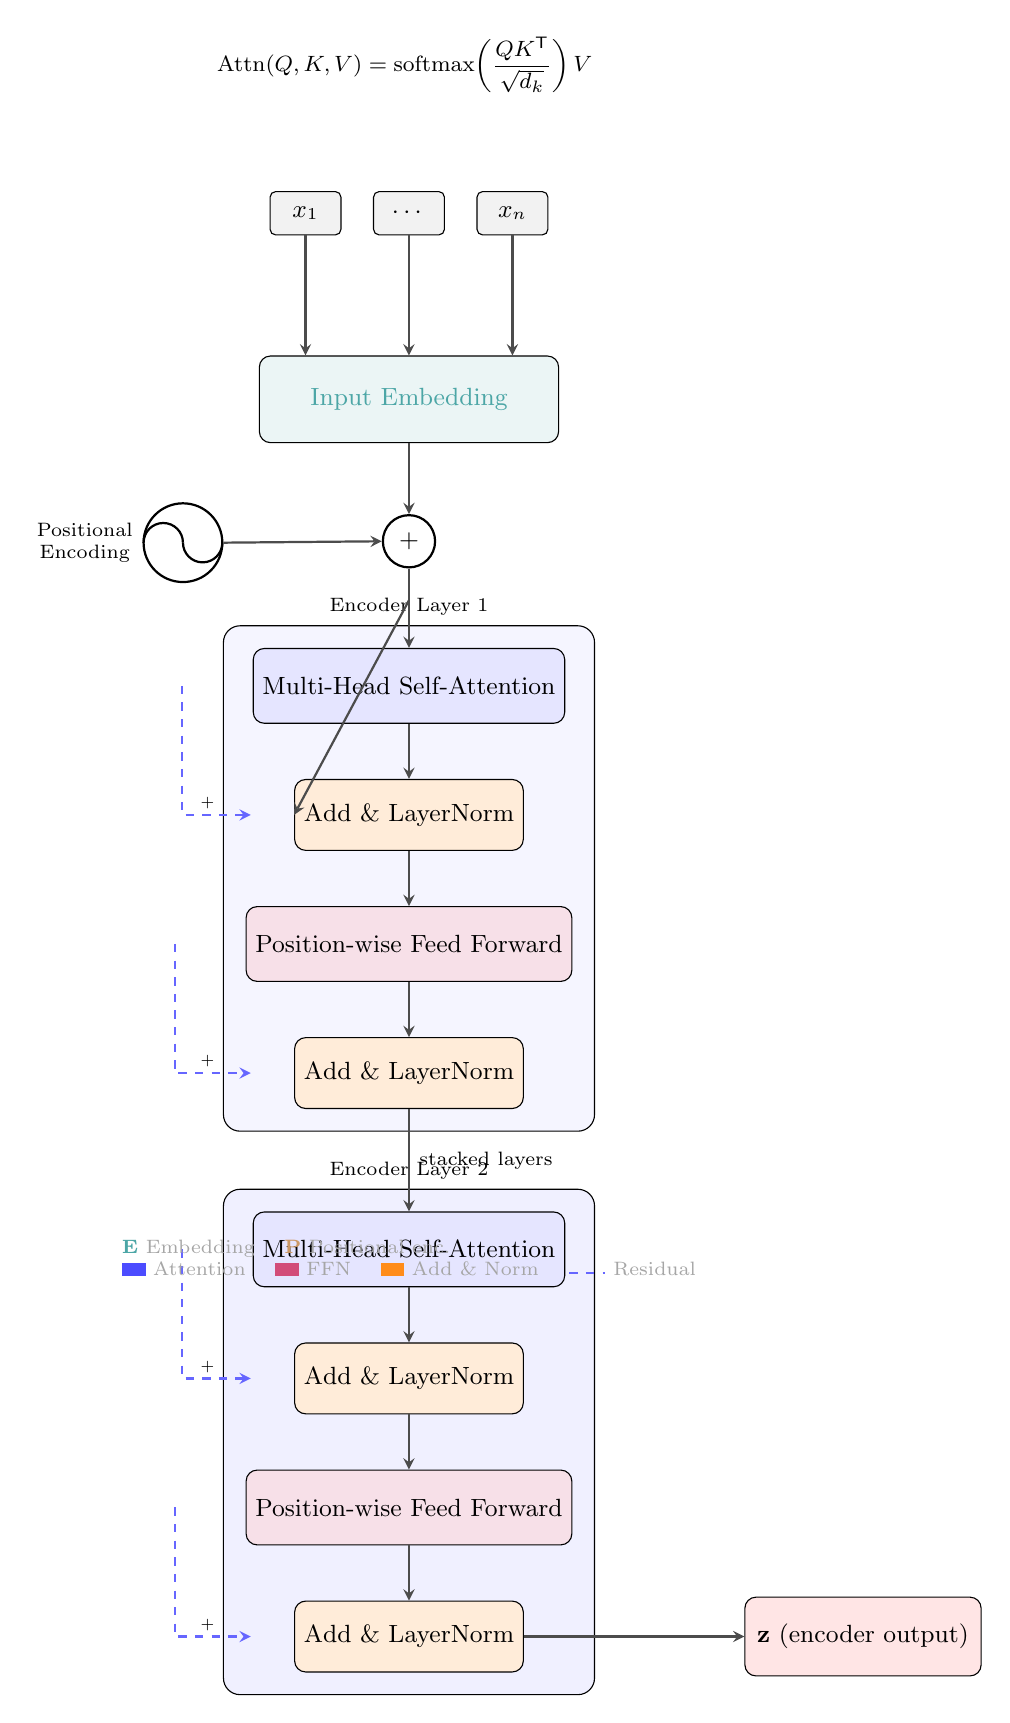
\begin{tikzpicture}[
        every node/.style={font=\small},
        node distance=0.7cm,
        token/.style={draw, rounded corners=2pt, minimum width=0.9cm, minimum height=0.55cm, fill=gray!10},
        embed/.style={draw, rounded corners=4pt, minimum width=3.1cm, minimum height=1.1cm, fill=teal!8},
        attn/.style={draw, rounded corners=4pt, minimum width=3.2cm, minimum height=0.95cm, fill=blue!10},
        norm/.style={draw, rounded corners=4pt, minimum width=2.8cm, minimum height=0.9cm, fill=orange!15},
        ffn/.style={draw, rounded corners=4pt, minimum width=3.2cm, minimum height=0.95cm, fill=purple!12},
        output/.style={draw, rounded corners=4pt, minimum width=3cm, minimum height=1cm, fill=red!10},
        arrow/.style={->, thick, >=stealth, draw=black!70},
        residual/.style={arrow, dashed, draw=blue!60},
        layerbox/.style={draw, rounded corners=6pt, inner sep=8pt}
    ]

    % Tokens
    \matrix[column sep=0.4cm] (tokens) {
        \node[token] (t1) {$x_1$};    &
        \node[token] (t2) {$\cdots$}; &
        \node[token] (t3) {$x_n$};      \\
    };

    % Input Embedding
    \node[embed, below=1.4cm of tokens, minimum width=3.8cm] (embed)
    {\textcolor{teal!70}{Input Embedding}};
    \coordinate (qtop) at (t1 |- embed.north);
    \coordinate (ktop) at (t2 |- embed.north);
    \coordinate (vtop) at (t3 |- embed.north);
    \draw[arrow] (t1.south) -- (qtop);
    \draw[arrow] (t2.south) -- (ktop);
    \draw[arrow] (t3.south) -- (vtop);

    % Positional Encoding
    \node[draw,circle,minimum size=1.0cm,line width=0.8pt] (pos)
    [label={[font=\scriptsize,align=center]left:{Positional\\Encoding}}]
    [below left=0.9cm and 0.6cm of embed] {};
    \draw[thick] ($(pos.center)-(0.5, 0)$) arc[start angle=180, end angle=0, radius=0.25cm];
    \draw[thick] ($(pos.center)+(0.5, 0)$) arc[start angle=0, end angle=-180, radius=0.25cm];

    % oplus
    \node[draw, circle, line width=0.8pt, below=0.9cm of embed] (oplus) {$+$};
    \draw[arrow] (pos.east) -- (oplus.west);

    % Encoder Layer 1
    \node[attn, below=2.6cm of embed] (mha1) {Multi-Head Self-Attention};
    \node[norm, below=0.7cm of mha1] (norm1) {Add \& LayerNorm};
    \node[ffn, below=0.7cm of norm1] (ffn1) {Position-wise Feed Forward};
    \node[norm, below=0.7cm of ffn1] (norm2) {Add \& LayerNorm};

    % Encoder Layer 2 (stacked)
    \node[attn, below=1.3cm of norm2] (mha2) {Multi-Head Self-Attention};
    \node[norm, below=0.7cm of mha2] (norm3) {Add \& LayerNorm};
    \node[ffn, below=0.7cm of norm3] (ffn2) {Position-wise Feed Forward};
    \node[norm, below=0.7cm of ffn2] (norm4) {Add \& LayerNorm};

    % Output
    \node[output, right=2.8cm of norm4] (out) {$\mathbf{z}$ (encoder output)};

    % Forward arrows
    \draw[arrow] (embed) -- (oplus);
    \draw[arrow] (oplus) -- node[pos=0.4, coordinate] (fork) {} (mha1);
    \draw[arrow] (fork.west) -- (norm1.west);
    \draw[arrow] (mha1) -- (norm1);
    \draw[arrow] (norm1) -- (ffn1);
    \draw[arrow] (ffn1) -- (norm2);
    \draw[arrow] (norm2) -- node[right=0.0cm, font=\scriptsize, align=left] {stacked layers} (mha2);
    \draw[arrow] (mha2) -- (norm3);
    \draw[arrow] (norm3) -- (ffn2);
    \draw[arrow] (ffn2) -- (norm4);
    \draw[arrow] (norm4) -- (out);

    % Residual paths
    \draw[residual] ([xshift=-0.9cm]mha1.west) |- ([xshift=-0.55cm]norm1.west);
    \draw[residual] ([xshift=-0.9cm]ffn1.west) |- ([xshift=-0.55cm]norm2.west);
    \draw[residual] ([xshift=-0.9cm]mha2.west) |- ([xshift=-0.55cm]norm3.west);
    \draw[residual] ([xshift=-0.9cm]ffn2.west) |- ([xshift=-0.55cm]norm4.west);
    \node at ([xshift=-1.1cm,yshift=0.15cm]norm1.west) {\tiny $+$};
    \node at ([xshift=-1.1cm,yshift=0.15cm]norm2.west) {\tiny $+$};
    \node at ([xshift=-1.1cm,yshift=0.15cm]norm3.west) {\tiny $+$};
    \node at ([xshift=-1.1cm,yshift=0.15cm]norm4.west) {\tiny $+$};

    % Layer backgrounds
    \begin{pgfonlayer}{background}
        \node[layerbox, fill=blue!4, fit=(mha1) (norm1) (ffn1) (norm2), label={[font=\scriptsize]above:Encoder Layer 1}] {};
        \node[layerbox, fill=blue!6, fit=(mha2) (norm3) (ffn2) (norm4), label={[font=\scriptsize]above:Encoder Layer 2}] {};
    \end{pgfonlayer}

    % Legend
    \node[align=left, font=\scriptsize, text=gray!70, below=10cm of embed] (legend) {
        \textcolor{teal!70}{\textbf{E}} Embedding \quad
        \textcolor{brown!80}{\textbf{P}} Positional enc. \\
        \textcolor{blue!70}{\rule{0.3cm}{0.16cm}} Attention \quad
        \textcolor{purple!70}{\rule{0.3cm}{0.16cm}} FFN \quad
        \textcolor{orange!90}{\rule{0.3cm}{0.16cm}} Add \& Norm \quad
        \tikz[baseline=-0.35ex]\draw[dashed,blue!60,thick] (0,0) -- (0.45,0); Residual
    };

    % Formula (optional reminder)
    \node[above=1cm of tokens, font=\footnotesize\itshape, align=center] {
        $\mathrm{Attn}(Q,K,V)=\operatorname{softmax}\!\left(\dfrac{QK^{\mathsf T}}{\sqrt{d_k}}\right)V$
    };

\end{tikzpicture}
\end{document}
